

\subsubsection{Memory virtualisation}
Modern Operating system use "memory paging" (the physical memory is interpreted into pages) to access as contiguous dispersed locations in the physical memory; the OS keeps a set of tables to translate the virtual memory address into physical ones (this operation is handled by \textbf{MMU}). Virtual addresses, used by processes (starting from 0), are translated by the MMU to physical addresses using big hash table for the mapping.




Another task of the MMU is to manage the \textbf{TLB} (\textit{Translation Lookaside Buffer}), a cache of recently used page translations with very fast access.

\begin{figure}[b]
    \centering
    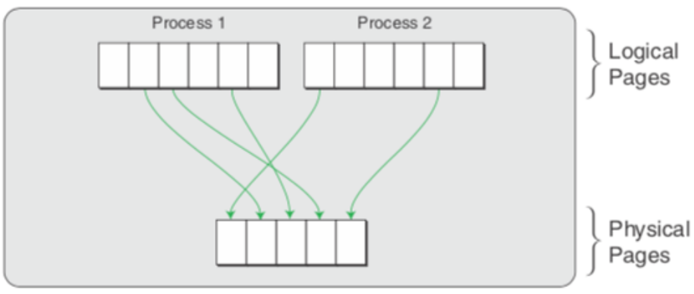
\includegraphics[scale=0.3]{images/mapping_mm.png}
    \caption{Mapping from LPNs to PPNs}
    \label{fig:mapping_mm}
\end{figure}

If we take a look at fig \ref{fig:mapping_mm} we see the walks that hardware does in order to determinate the corresponding physical address. for faster access hardware caches the most recently used LPN-$>$PPN mappings into TLB.

But why we virualize memory?
\begin{itemize}
    \item \textbf{Simplicity}: Every process gets illusion of whole address space (apps doesn't care of pages ecc.).
    \item \textbf{Isolation}: Every process is protected from every other.
    \item \textbf{Optimization}: Reduces space requirements (optimize the way of using the pages).
\end{itemize}
In VMs is required another level of translation (Guest virtual address -> Guest physical address -$>$ Machine physical address). To avoid this step a "\textbf{Shadow Page Table}" is introduced: it stores and keep track of the mapping between Guest logical address and Machine pysical pages, it's invisible from the guest point of view and it'll be used by the CPU for a traslation when the guest is active.

How it works:
\begin{itemize}
    \item PPN-$>$MPN manteined by VMM in internal data structures.
    \item LPN-$>$MPN stored by VMM in shadow page table expsed to hardware.
    \item Most recently used LPN-$>$MPN in hardware TLB.
\end{itemize}
\begin{figure}
    \centering
    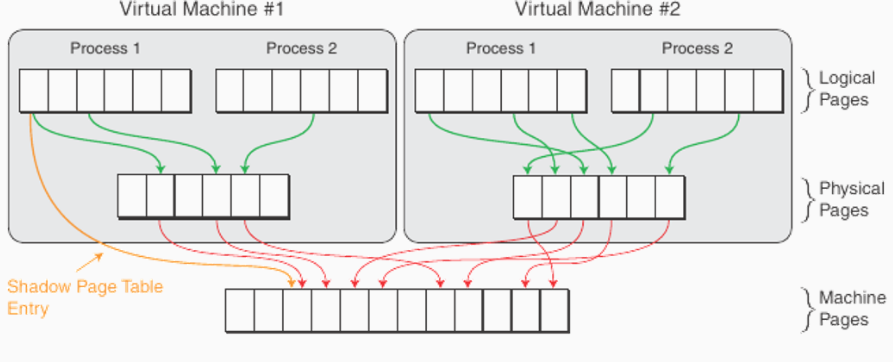
\includegraphics[scale=0.3]{images/mapping2_mm.png}
    \caption{CPU see only orange arrows, VMM see only the red ones}
    \label{fig:mapping2_mm}
\end{figure}
The VMM is in charge of keeping the Shadow Page Table synchronized with the guest OS page table, an important problem is the extra overhead is introduced in presence of page faults. In order to avoid this overhead Intel and AMD introduces Extended Page Table (or Rapid Virtualisation Indexing): traditional page tables translate LPN-$>$PPN, VMM maintains PPN->MPN mappings in an additional level of page tables, called \textbf{nested}.
\begin{itemize}
    \item Both the traditional page tables and the nested page tables are exposed to the CPU (now CPU know all the "path").
    \item Now there's no need to expose Shadow Page Tables, CPU does all the work (fig. \ref{fig:mapping3_mm})
\end{itemize}
\begin{figure}
    \centering
    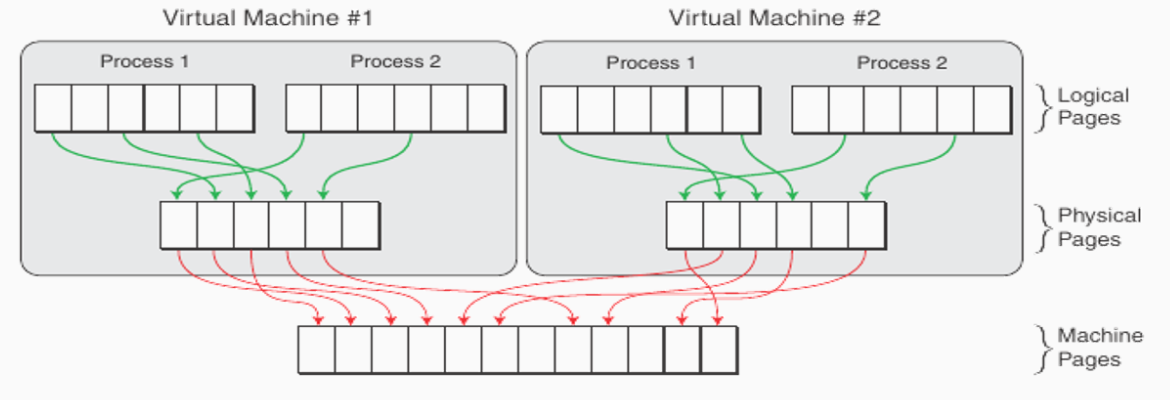
\includegraphics[scale=0.3]{images/mapping3_mm.png}
    \caption{Extended Page Table}
    \label{fig:mapping3_mm}
\end{figure}
This approach removes the need od VMExit (A context switch) associated with page table virtualisation, guest could now keep update its page table without any overhead. In addition to this now theres no need to use Shadow Page Table anymore but this increases the cost of a single page walk, now TLB cache becomes critical to guarantee good performance (in Intel processors theres two TLB, one for normal pages and one for huge pages). One last step to optimize \textbf{EPT} is to add an identifier for each virtual processor, this technique allows several virtual processors coexist on the TLB at the same time!
\subsubsection{I/O virualisation}
Like the other resources, there are several techniques adopted for virtualizing I/O devices
\begin{itemize}
    \item Device emulation
    \item Para-virtualized device
    \item Direct assignment
\end{itemize}
The choice of the technique depends on the type of device and if it Shared/Dedicated to a single Guest OS. We know that I/O communicate with the OS thanks to the \textbf{drivers\footnote{they standardise the method for the communication}}.

In \textbf{Device emulation} VMM proposes to the Guest OS an emulated device, guest OS has no idea that is an emulated device and the VMM has to remap device communication with the physical device in real OS (VMM has to emulate the response of the I/O for the Guest OS, Guest OS doesn't care to the real drivers).
It's like a trap n' emulate.
This approach is simple and easy to set up, there's no need to install dedicated drivers and a single physical device could be multiplexed with several emulated device. But I/O operation are generally slower than physical ones and that could increase substantially the CPU load.

In \textbf{Para-virtualized device} Guest OS is enriched with dedicated drivers (Guest OS knows that it's virtualised), is very similar to the CPU one but in this case is simpler, it require only to create dedicated device drivers instead of modifing a kernel (this approach make things easyer and faster). Some examples of PV drivers are Network cards, Disks, Graphical video card and shared memory. Besides the traditional drivers there are some special ones like the Memory Ballooning. This one is to create a "dynamic" memory, the driver provides to the hypervisor the information about current memory occupation of the guest, this allows the hypervisor to over-commit memory allocation to several guests.

In \textbf{direct assignment}










% ------------------------------------------



In Linux all processes are generated by a \textit{fork()} function invoking starting from the \textit{init()\footnote{nowadays called \textit{systemd}}} process. So processes generate other processes, creating a tree. A process with enough privileges and under some conditions can inspect another process by attaching a tracer to it or may kill/suspend it.

PID namespace enable multiple nested process tree (fig. \ref{fig:nestedtree}), the nested process think it's the "init" one (PID 1) this thanks to the isolation. The parent PID namespace know about all the processes but the child one doesn't know about the processes in the yellow area. So a single process can now have multiple PIDs associated to it this because they are associated with the corresponding namespace.

\begin{figure}
    \centering
    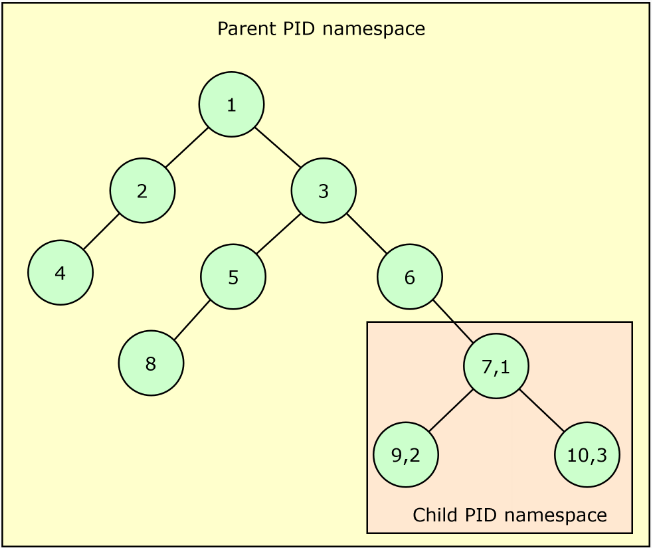
\includegraphics[scale=0.4]{images/processtree.png}
    \caption{An example of nested process with isolation}
    \label{fig:nestedtree}
\end{figure}

We saw that there are different namespaces for different kind of uses. Let's talk about \textbf{network namespace}. The network namespace allows two processes to perceive a completely different network setup (like routing table, interfaces, firewall, loopback ecc.). Once a network namespace is created we should create additional virtual network interfaces, these allows traffic to cross the namespace borders and be delivered to another namespace (fig. \ref{fig:netnamespace}).

An example:
\begin{verbatim}
    sudo ip netns add <netsname> #create a new network namespace named <netsname>
    sudo ip link add veth0-root type veth peer name veth0-ns # Create virtual eth links
    sudo ip link set veth0-ns netns <netsname>
\end{verbatim}
To interact in the namespace use the command
\begin{verbatim}
    [sudo] ip netns exec <namespace_name> <command>
\end{verbatim}

Other example of namespaces are \textbf{Mount namespace}, that enable the creation of a completly new file system, the \textbf{User namespace} that allows a process to have root privileges and another is the \textbf{IPC namespace} that creates private inter-process communication.
\begin{figure}
    \centering
    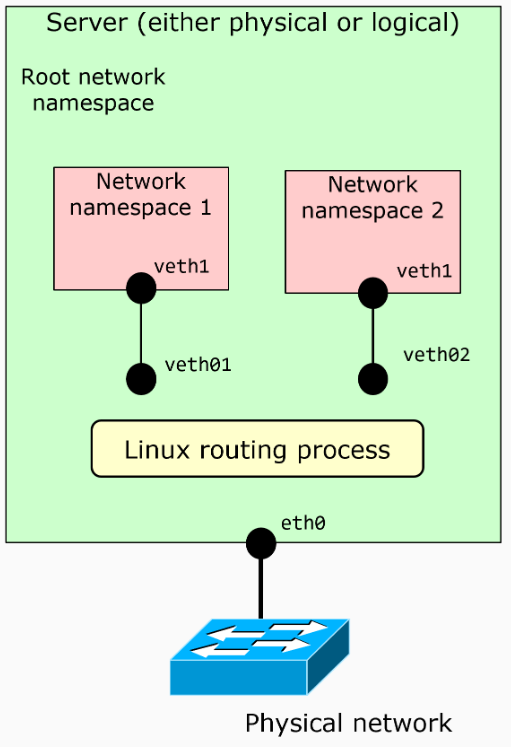
\includegraphics[scale=0.5]{images/netnamespace.png}
    \caption{Schema of a basic network namespace}
    \label{fig:netnamespace}
\end{figure}

\subsubsection{Limitation of these approaches}
Cgroups and Namespaces have some limitations beyond process isolation, they can provide a solution for a single server but it takes a lot of command to handle an entire datacenter and they cannot guarantee application portability (such as in case of VMs).

\subsubsection{Linux containers}
A solution for the cgroups and namespaces problem are the \textbf{linux containers}, they can provide lightweight virtualisation (isolation without the complexity of full virtualisation). Is an OS-level virtualisation method for running multiple isolated Linux systems on a single control host (the linux kernel is shared across all containers). Let's see the differences between Containers and Hypervisors, kernel is pretty small compared with the libs and bins in an OS, it can be shared because it's rare that one app need a specific kernel. In term of performance for the \textbf{CPU} the bet choice is containers, for the \textbf{memory} containers to and for the \textbf{storage} there are no differences. 

Containers share the same operating system (kernel) as the host, inside the box they look like a VM (or better a machine), but outside the box they look like normal processes. They don't emulate hardware and don't run different kernels and most important, security is not an out-of-the-box feature. Containers are faster and lighter than real VM (they can achieve the same performances of native execution) but in the other hand the VMs provide better isolation, better security and give the possibility to use different OSs.

An overkill feature of the containers is that they are versatile.
\begin{figure}
    \centering
    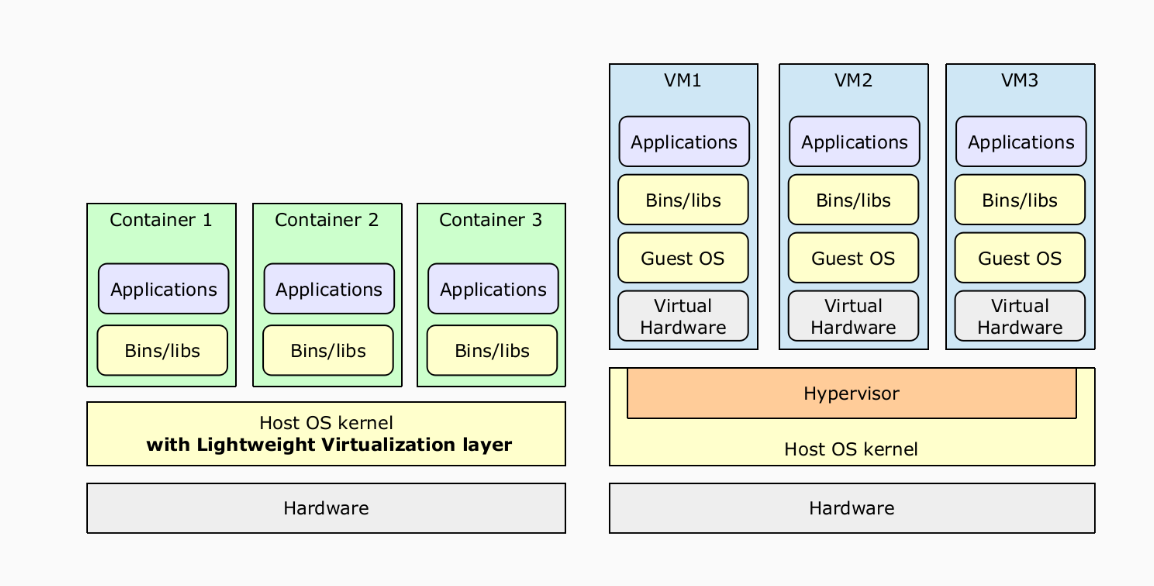
\includegraphics[scale=0.30]{images/contvshyp.png}
    \caption{Containers vs Hypervisors}
    \label{fig:cvs}
\end{figure}
\subsubsection{LXC}